% ============================================ %

\documentclass[14pt,a4paper]{extarticle}
%\documentclass[12pt,a4paper]{article}

\usepackage[utf8]{inputenc}
\usepackage[ukrainian]{babel}


\usepackage{amssymb}
\usepackage{physics}
\usepackage{amsmath}
% \operatorname*{argmin}_\theta f(x)
% \operatorname*{arg\,max}_\theta f(x)



\usepackage[active]{srcltx}
\usepackage[final]{pdfpages}

\usepackage[hidelinks]{hyperref}

\usepackage{verbatim}

\usepackage{algpseudocode}
\usepackage{algorithm}
\floatname{algorithm}{Algorithm}
\renewcommand{\algorithmicrequire}{\textbf{Input: }}
\renewcommand{\algorithmicensure}{\textbf{Output: }}
\newcommand{\algorithmreturn}{\textbf{return }}

% ============================================ %

%\pagestyle{empty}                     %нумерацiя сторiнок i т.д.
\pagestyle{headings}                   %нумерацiя сторiнок вгорi зправа i т.д.
%\renewcommand{\baselinestretch}{1.5}   %мiжстрiчковий інтервал
%\parindent=7.5mm                      %абзацний відступ
\righthyphenmin=2                     %перенос 2 останніх букв
\pagenumbering{arabic}
\tolerance=400
\mathsurround=2pt
\hfuzz=1.5pt

% ============================================ %

\hoffset=-0.5cm        %+2.5cm -- вiдступ вiд лiвого краю
\voffset=-1.5cm        %+2.5cm -- вiдступ зверху
\oddsidemargin=0.1cm   %ліве поле
\topmargin=0.1cm       %верхнє поле
\headheight=0.5cm      %висота верхнього колонтитулу
\footskip=1cm          %висота нижнього колонтитулу
\headsep=0.3cm         %відступ від колонт. до тексту
\textwidth=17cm        %ширина сторінки
\textheight=25.5cm     %висота сторінки

% ============================================ %
	
\newcounter{e}
\setcounter{e}{0}
\newcommand{\n}{\refstepcounter{e} (\arabic{e})}

\newcounter{pic}
\setcounter{pic}{0}
\newcommand{\pic}[1]{\refstepcounter{pic} \vspace{-0.3cm}\textit{Рисунок \arabic{pic}\label{#1}.}}

\newcounter{tabl}
\setcounter{tabl}{0}
\newcommand{\tabl}[1]{\refstepcounter{tabl} \vspace{-0.3cm}\textit{Таблиця \arabic{tabl}\label{#1}.}}

\newcounter{dod}
\setcounter{dod}{0}
\newcommand{\dod}[1]{\refstepcounter{dod} \textit{Додаток \arabic{dod}\label{#1}.}}




\newtheorem{theorem}{Теорема}[section]
\newtheorem{defn}[theorem]{Означення}
\newtheorem{lemma}[theorem]{Лема}

\newcommand{\proof}{\textit{Доведення. \space}}
% \setcounter{page}{1}
% \setcounter{section}{1}

\numberwithin{equation}{section}
\numberwithin{figure}{section}


% \newcommand{\unknownx}{	\boldsymbol{$1}^{\star}}
% \newcommand{\bt}[1]{\textbf{#1}}
% custom commands
\newcommand{\tran}{^{T}}
\newcommand{\ith}{^{(i)}}
\newcommand{\lth}{^{(l)}}




% ============================================ %
	
% bibliography
\usepackage[
	backend=biber,
	style=numeric,
	sorting=none
]{biblatex}
\addbibresource{resources/bibliography.tex}

% ============================================ %

\begin{document}
	% ============================================ %
	\begin{titlepage}%
		\begin{center}
			{\textbf{ЛЬВІВСЬКИЙ НАЦІОНАЛЬНИЙ УНІВЕРСИТЕТ \\ ІМЕНІ ІВАНА ФРАНКА}}\par
			{Факультет прикладної математики та інформатики \\ Кафедра обчислювальної математики}\par
			\vspace{40mm}
			{\textbf{\huge{Кусова робота}}}\par
			\vspace{5mm}
			{\large{Використання глибокого навчання для обернених задач}}\par
			\vspace{5mm}\par %subtitle
		\end{center}
		
		\vfill
		\vskip80pt
		
		\begin{flushleft}
			\hskip 8cm 
			Виконав студент IV курсу групи
			\\ \hskip8cm
			ПМп-41 напрямку підготовки 
			\\ \hskip8cm
			(спеціальності)
			\\ \hskip8cm
			113 -- ``Прикладна математика''
			\\ \hskip8cm
			Середович В.B.
		\end{flushleft}
		\begin{flushleft}
			\hskip8cm 
			Керівник: Музичук Ю.А.
		\end{flushleft}
		
		\vfill
		
		\begin{center}
			\large
			Львів - 2021
		\end{center}
	\end{titlepage}

	% ============================================ %
	% Зміст
	\addtocontents{toc}{\protect\thispagestyle{empty}}
	\tableofcontents

	% ============================================ %
	% Вступ
	
	\newpage
	\thispagestyle{empty}
	\addcontentsline{toc}{section}{Вступ}
	\section*{Вступ}
	Оберненими задачами називають такі задачі, в яких необхідно відновити дані про деякий процес з використанням непрямих спостережень. Такі спостереження отримують за допомого певного прямого процесу який, зазвичай, є необоротнім, а отже не має єдиного розв'язку. Як наслідок, задачі такого типи можуть бути нерозв'язними без додаткової інформації про задачу. До таких погано обумовлених задач можна віднести багато прикладів з реальних фізичних процесів, таких як задачі сейсморозвідки на основі звукових сигналів або багато задач із зображеннями, такі як реконструкція рентгенівської або акустичної томографії, видалення шуму, збільшення розмірності, заповнення втрачених даних в зображеннях та інші. 
	
	Класичний підхід до розв'язання таких задач припускає наявність певної попередньої інформації про обернену задачу на основі якого будується прямий оператор та функціонал регуляризації з яких формується задача мінімізації.
		
	Однак, за останій час алгоритми глибокого навчання набирають значну популярність в області розв'язуванні обернених задач через свою ефективність, та універсальність для багатьох різних типах задач. \cite{ongie2020deep}. 
	
	Отже в межех цієх роботи будемо розглядати деякі методи по реконструкції зображень на основі глибокого навчання та проаналізуємо їх ефективність.
	% ============================================ %
	
	\newpage
	\thispagestyle{empty}
	\section{Постановка задачі} 
	
	
	\begin{comment}
	"""
	Відповідно до поняття, уведеного на початку століття Ж. Адамаром, задачу
	z  Ru називають коректно поставленою, якщо вона задовольняє тр и умови:
	1) за кожного u U розв'язок задачі існує;
	2) розв'язок є єдиний за кожного u U ;
	3) розв'язок є стійкий до малих варіацій величини u , тобто достатньо малим
	зміненням величини u відповідають як завгодно малі зміни величини z [1, 7].
	Якщо задача не задовольняє хоча б одну із зазначених умов, то її називають некоректно поставленою.
	Очевидно тепер, що обернені задачі в розглянутих прикладах відносять до
	числа некоректно поставлених, оскільки в них порушується третя, а мо жливо, і
	перша із зазначених вище умов. Некоректність постановки обернен ої задачі і є її
	математична особливість. Якщо для пошуку наближеного розв’язку оберненої з адачі застосовувати будь-який класичний алгоритм формально, не враховуючи н екоректність постановки задачі, то є великий ризик отримати результат, який не
	має ні наукової, ні прикладної цінності.
	"""
	\end{comment}
	
	
	
	
	Оберненими задачами будемо вважати такі задачі, в яких невідомим є $n-$ піксельне зображення $\boldsymbol{x} \in \mathbb{R}^{n}$ яке було отримане з $m$ вимірювань $\boldsymbol{y} \in \mathbb{R}^{m}$ відповідно до рівняння
	\begin{equation}
	\label{forward-problem}
	\boldsymbol{y}=\mathcal{A}\left(\boldsymbol{x}\right)+\boldsymbol{\varepsilon}
	\end{equation}
	де $\mathcal{A}$ - це прямий оператор вимірювання та $\boldsymbol{\varepsilon}$ є певним вектором шуму. Метою задачі є відновлення $x$ з $y$. Можна розглянути більш загальний випадок моделі неадитивного шуму, який має вигляд 
	\begin{equation}
	\label{forward-problem-non-additive}
	\boldsymbol{y}=\mathcal{N}\left(\mathcal{A}\left(\boldsymbol{x}\right)\right)
	\end{equation}
	де $\mathcal{N}(\cdot)$ є прикладами вибірки з шумом.


	\begin{defn}
		\label{well-posed}
		Відповідно до поняття, уведеного Жаком Адамаром, задачу \ref{forward-problem-non-additive} називають коректно поставленою, якщо вона задовольняє наступні умови: 
		\begin{enumerate}
			\item Для кожного $x$ розв'язок задачі існує.
			\item Розв'язок є єдиний для кожного $x$.
			\item Розв'язок є стійкий до малих варіацій величини $x$, тобто достатньо малим зміненням величини $x$ відповідають як завгодно малі зміни величини $y$.
		\end{enumerate}
	\end{defn}

	\begin{defn}
		\label{ill-posed}	
		Задачу, яка не задовольняє хоча б одну з умов означення \ref{well-posed}, називають некоректно поставленою.
	\end{defn}

	Тому, очевидно, що розглянута обернена задача є некоректно (або погано обумовленою), оскільки в ній порушуються умови означення \ref{well-posed}. Така задача знаходження єдиного розв'язку, яка задовольняє спостереженням є складною або неможливою, за умови відсутності попередніх знань про дані.

	Оцінку справжнього зображення $\boldsymbol{x}$ з $\boldsymbol{y}$  вимірювання називають задачею реконструкції зображення. Класичні підходи до реконструкції зображень припускають наявність деякої попередньої інформації про зображення, яку називають пріором. В якості пріору можуть виступати параметри гладкості, щільності та інші геометричні властивості зображення.

	%TODO
	Отже, метою даної роботи буде розв'язання таких обернених задач за допомогою алгоритмів глибокого навчання. Зокрема, будемо розглядати проблему видалення шуму у зображеннях.

	% ============================================ %
	\newpage
	\thispagestyle{empty}
	\section{Структура обернених задач}

	%\subsection{Розв'язування обернених задач}
	Відповідно до постановки задачі, ми прагнемо відновити векторизоване зображення $\boldsymbol{x} \in \mathbb{R}^{n}$ з вимірювань $\boldsymbol{y} \in \mathbb{R}^{m}$ у вигляді $\boldsymbol{y}=\mathcal{A}\left(\boldsymbol{x}\right)+\boldsymbol{\varepsilon}$.

	Якщо розподіл шуму відомий, $x$ можна відновити розв'язавши задачу оцінки максимальної ймовірності (maximum likelihood):
	$$
	\hat{\boldsymbol{x}}_{\mathrm{ML}}
	= \arg \max_{\boldsymbol{x}} {p (\boldsymbol{y} \mid \boldsymbol{x})}
	= \arg \min_{\boldsymbol{x}} -\log p(\boldsymbol{y} \mid \boldsymbol{x})
	$$
	де $p(\boldsymbol{y} \mid \boldsymbol{x})$ це ймовірність спостереження $\boldsymbol{y}$ за умови якщо $\boldsymbol{x}$ є справжнім зображенням.
	
	В залежності від умов задачі, можуть бути відомі попередні дані про те яким має бути $x$. Ці умови можна для формування  задачі оцінки максимальної апостеріорної ймовірності (maximum a posteriori), що приводить до задачі
	
	$$
		\hat{\boldsymbol{x}}_{\mathrm{MAP}}
		=
		\arg \max_{\boldsymbol{x}} p(\boldsymbol{x} \mid \boldsymbol{y}) 
		=
		\arg -\max_{\boldsymbol{x}} { p(\boldsymbol{y} \mid \boldsymbol{x})} p(\boldsymbol{x})
		=
		\arg \min_{\boldsymbol{x}} -\ln p(\boldsymbol{y} \mid \boldsymbol{x})-\ln p(\boldsymbol{x})
	$$
	
	Для випадку білого гаусівського шуму, цільову функцію можна сформулювати як:
	\begin{equation}
		\label{MAP-avgn}
		\hat{x}=\arg \min_{x} 	\frac{1}{2}\|\mathcal{A}(\boldsymbol{x})-\boldsymbol{y}\|_{2}^{2}+\lambda \mathrm{R}(\boldsymbol{x})
	\end{equation}
	де  $|\mathcal{A}(\boldsymbol{x})-\boldsymbol{y}\|_{2}^{2}$ відповідає за правдивість даних та позначає різницю між вихідним та шумним зображеннями, $\mathrm{R}(\boldsymbol{x})$ є пропорційним до від'ємного логарифмічного пріора та позначає член регуляризації, а $\lambda$ є параметром регуляризації. Для варіаційних методів видалення шуму, ключовим є пошук відповідного пріору зображення $\mathrm{R}(\boldsymbol{x})$. Варіантами таких пріорів моделі можуть бути градієнтні або розріджені пріори.

	Прикладом такого підходу до розв'язування некоректних задач є метод регуляризації Тіхонова. Він базується на мінімізації параметра регуляризації $\mathrm{R}_{\mathrm{TR}}$ за $L_2$ нормою, який можна подати у вигляді \ref{tikhonov-reg-parameter}.
	
	\begin{equation}
		\label{tikhonov-reg-parameter}
		\mathrm{R}_{\mathrm{TR}}(\boldsymbol{x})
		=
		\|\nabla \boldsymbol{x}\|_{2} 
		=
		\sqrt{\left|\nabla_{v} x\right|^{2}+\left|\nabla_{h} x\right|^{2}}
	\end{equation}
	де $\nabla_{h} \boldsymbol{x}$ та $\nabla_{v} \boldsymbol{x}$ є операторами градієнта по горизонталі та вертикалі зображення відповідно.
	
	%% cite https://www.hindawi.com/journals/am/2014/934834/	
	Задача максимальної апостеріорної оцінки може використовуватись для реконструкції зображень, однак такий підхід може бути не таким ефективним, якщо розподіл шуму або прямий оператор $\mathcal{A}$ є невідомі.  
	Алгоритми основані на використанні машинного навчання дають змогу побороти більшість з цих труднощів, що робить їх ефективною альтернативою класичному підходу.

	%\subsection{Огляд машинного навчання для розв'язування обернених задач}

	% ============================================ %
	\newpage
	\thispagestyle{empty}
	\section{Використання глибокого навчання для обернених задач}

	\subsection{Контрольоване і неконтрольоване навчання}
	Перший і найпоширеніший тип розв'язування обернених задач з використанням глибокого навчання є контрольована інверсія. Ідея полягає у створенні співвідношення між датасетом справжніх зображень $x$ та відповідними вимірюваннями $y$. Тобто ми можемо натренувати нейронну мережу приймати значення $y$ та реконструювати оберенне значення $x$. Цей підхід є дуже ефективним, однак є чутливим до змін в операторі вимірювання $A$. 
	
	Другим типом розв'язування обернених задач є неконтрольованого навчання. Він передбачає, що інформація про пари вхідної та вихідної інформації $x$ та $y$ невідомі під час тренування. До нього можна віднести ситуації коли відомі тільки справжні зображення $x$ або тільки результати вимірювання $y$.
	
	Ці два підходи мають фундаментальні відмінності та ця робота націлена саме на методи контрольованого навчання, тому що очікується, що вони дадуть кращі результати в порівнянні з класичними методами. 
	
	\subsection{Класифікація навчання розв'язування обернених задач}
	
	Відповідно до \cite{ongie2020deep} існує багато варіантів застосування глибокого навчання для розв'язування обернених задач. Більшість з них можна поділита на декілька груп:
	\begin{itemize}
		\item \textbf{Пряма модель $\mathcal{A}$ є відома під час тренування та тестування} \newline
		Для цьогу випадку найбільш доцільним підходом є використання контрольованих моделей машинного навчання, тому що маючи доступ до оригінальних зображень та прямого оператора можна легко згенерувати пари для тренування моделі.
				
		\item \textbf{Пряма модель $\mathcal{A}$ є відома тільки під час тестування} \newline
		Для таких алгоритмів характерно, що якщо один раз навчити глибоку моделі, цю ж саму модель можна буде використовувати для будь-якої іншої прямої моделі. Це вигідно в ситуаціях, коли оригінальних зображень є достатньо, але навчання глибоких нейроних мереж для різних прямих моделей є недоцільно.

		\item \textbf{Пряма модель $\mathcal{A}$ є відома тільки частково} \newline
		Це може статися, наприклад, коли пряма модель є параметричною, і ми знаємо або розподіл, або
		достатню статистику про параметри.

		\item \textbf{Пряма модель $\mathcal{A}$ є невідома} \newline
		У деяких випадках пряма-модель може бути абсолютно невідомою, неправильно визначеною або обчислювально неможливою для використання в навчанні та тестуванні. Тоді навчання може відбуватись лише з відповідними парами зображень та вимірювань. 
	\end{itemize}

	\newpage
	\thispagestyle{empty}
	\section{Автоенкодер для розв'язування обернених задач}

	Одним з методів до розв'язування обернених задач на основі глибокого навчання є нейрона мережа автоенкодер яка може використовуватись у випадку коли пряма модель $\mathcal{A}$ та чисті зображення є відомі, або коли є достатня кількість пар чистих та пошкоджених зображень для тренування нейронної мережі.

	\subsection{Автоенкодер}
	
	Автоенкодером називають нейрону мережу яка навчається копіювати свої вхідні дані у вихідні. Така мережа має проміжний шар $h$, також відомий як латентний, який зберігає параметри необхідні для представлення вхідних даних. Таку нейрону мережу можна подати у складі двох частин: функції енкодера $h = f(x)$ та декодера який відтворює $r = g(h)$. Ця архітектура подана на зображенні \ref*{fig:autoencoder-graph}.
	\begin{figure}[h]
		\centering
		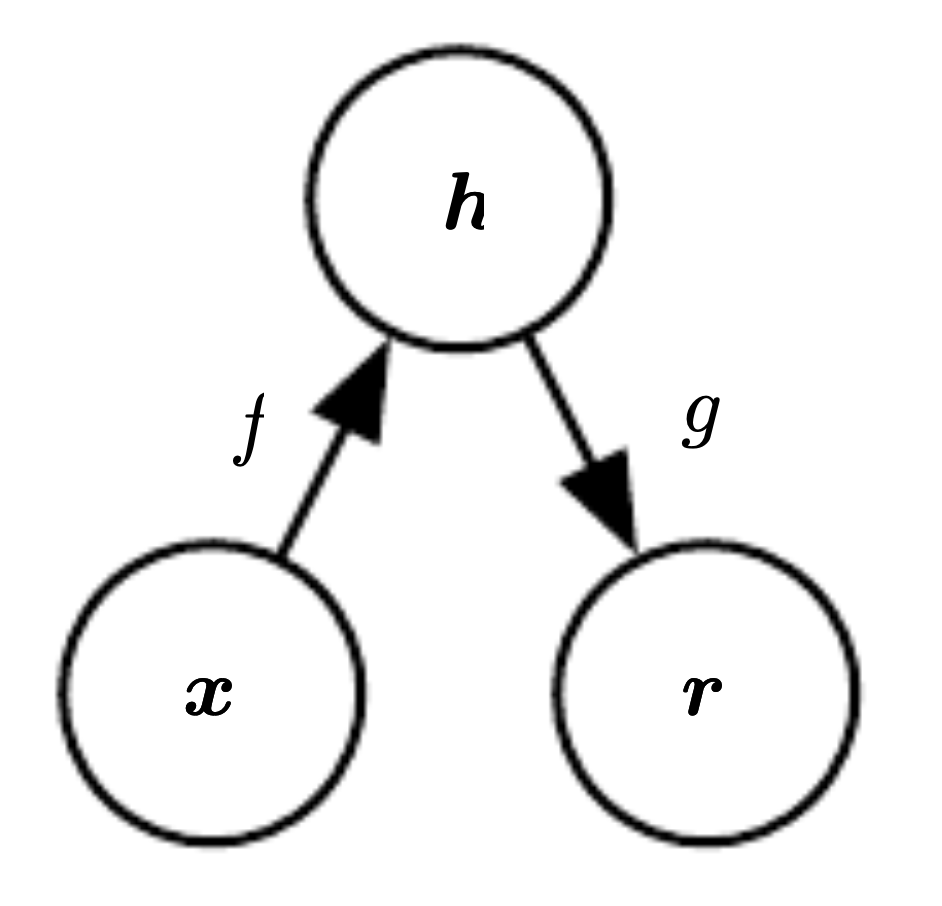
\includegraphics[width=0.3\textwidth]{resources/autoencoder_graph.png}
		\caption{Загальна структура автокодера, що відображає вхід $x$ на вихід $r$ (реконструкцію) через внутрішнє представлення $h$. Автокодер складається з двох компонентів: енкодера $f$ (відображення $x$ до $h$) та декодера $g$ (відображення $h$ до $r$) \cite{Goodfellow-et-al-2016}} 
		\label{fig:autoencoder-graph}
	\end{figure}
	Якщо автоенкодеру вдається навчитися просто відтворювати $g(f(x)) = x$ для всіх прикладів, то це не має особливої користі. Тому автоенкодери зазвичай обмежують таким чином, щоб вони не могли відтворювати ідеальну копію вхідних даним.
	
	\subsection{Автоенкодер для видалення шуму}
	Класичні автоенкодери мінімізують деяку функцію:
	\begin{equation}
		L(\boldsymbol{x}, g(f(\boldsymbol{x})))
	\end{equation}
	де $L$ це штрафна функція яка карає $g(f(\boldsymbol{x}))$ за відмінність від $\boldsymbol{x}$, таку як $L^{2}$ норму від їх різниці. В результаті це призводить до того, що композиція функцій $g \circ f$ навчається бути тотожнім відображення якщо для того є можливість. На відміну від цього, автоенкодер для видалення шуму мінімізує:	
	\begin{equation}
		L(\boldsymbol{x}, g(f(\tilde{\boldsymbol{x}})))
	\end{equation}
	де $\tilde{\boldsymbol{x}}$ є копією $\boldsymbol{x}$ який був пошкоджений деяким шумом. 
		
	Отже, такий автоенкодер має відновити пошкодження, натомість простому відтворенню вхідних даних. Процес тренування автоенкодера заданий на \ref{fig:dae-graph}.
	\begin{figure}[h]
		\centering
		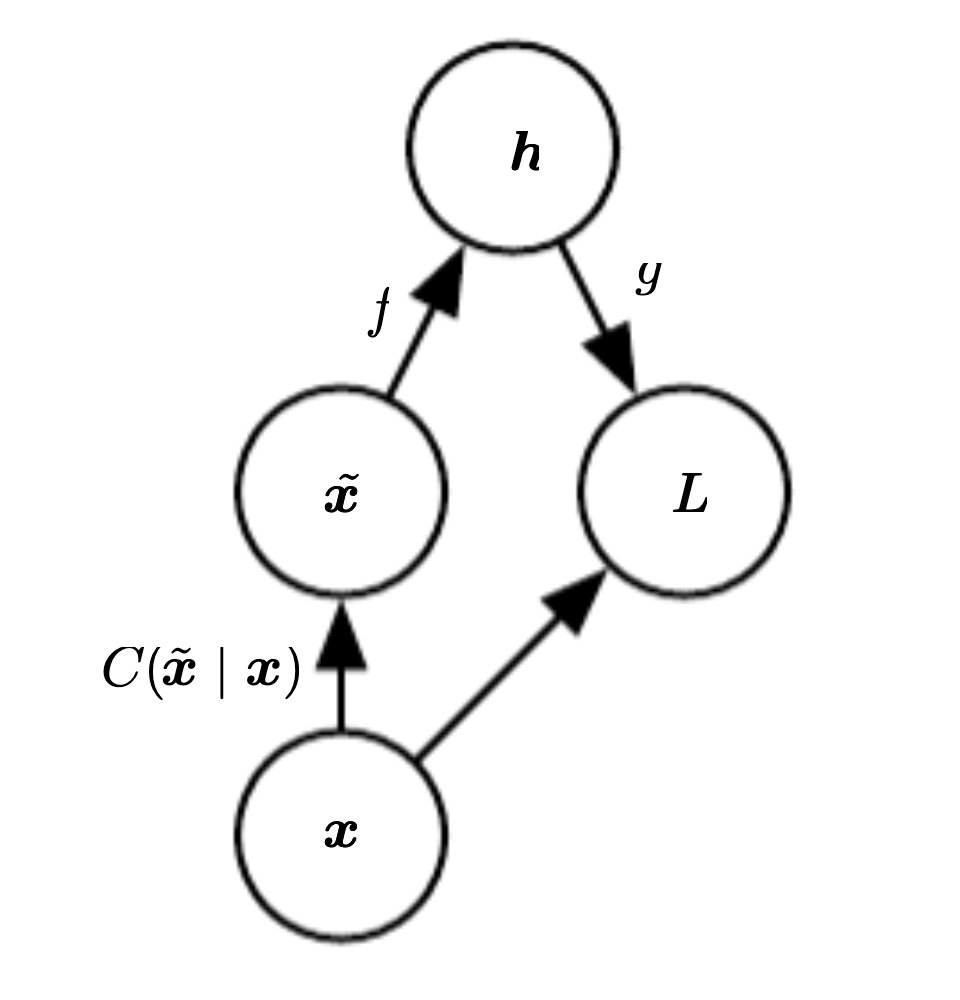
\includegraphics[width=0.4\textwidth]{resources/dae_graph.png}
		\caption{
			Структура функції витрат для автоенкодера який навчається реконстроювати чисті зображення $x$ з пошкождених. Тренування виконується на основі мінімізації функції втрат: $\tilde{x}$.  $L = - \log p (\boldsymbol {x} \mid \boldsymbol {h} = f (\tilde {\boldsymbol {x}}))$, де $\tilde {\boldsymbol {x}}$ - пошкоджена версія прикладу $\boldsymbol {x}$, отримана в результаті деякого процесу руйнування $C (\tilde {\boldsymbol {x}} \mid \boldsymbol {x})$. \cite{Goodfellow-et-al-2016}
		}
		\label{fig:dae-graph}
	\end{figure}
		
	Такий підхід до навчання видалення шуму змушує $f$ та $g$ явно вивчати структуру даних що дозаоляє ефективно використовувати автоенкодер для задач.

	\subsection{Варіаційний автоенкодер для видалення шуму}

	% ============================================ %		
	\newpage
	\section{Модель глибокої нейронної мережі}

	Нехай маємо набір тренувальних даних:
	\begin{equation*}
		(x^{(1)}, y^{(1)}), \quad (x^{(2)}, y^{(2)}), \quad ... \quad ,(x^{(m)}, y^{(m)})
	\end{equation*}
	\begin{equation*}
		\quad
		x =	
		\begin{bmatrix}
			\vdots  & \vdots  & & \vdots \\
			x^{(1)} & x^{(2)} &   \dots & x^{(m)}\\
			\vdots  & \vdots  & & \vdots
		\end{bmatrix}
		\quad
		x\ith \in
		\begin{bmatrix}
			x\ith_1   \\
			\vdots \\
			x\ith_n
		\end{bmatrix}
		\quad
	\end{equation*}
	\begin{equation*}
		\quad
		y =	
		\begin{bmatrix}
			\vdots  & \vdots  & & \vdots \\
			y^{(1)} & y^{(2)} &   \dots & y^{(m)}\\
			\vdots  & \vdots  & & \vdots
		\end{bmatrix}
		\quad
		y\ith \in
		\begin{bmatrix}
			y\ith_1   \\
			\vdots \\
			y\ith_n
		\end{bmatrix}
		\quad
	\end{equation*}
	де
	\begin{itemize}
		\item $x$ - матриця в якій кожен $i-$ий стовпець є розгорнутим у вектор справжнього зображення, $i=1,\dots,m$
		\item $y$ - матриця в якії кожен $i-$ий стовпець є розгорнутим у вектор пошкодженого зображення
		\item $m$ - кількість прикладів
		\item $n$ - кількість характеристик в кожному прикладі (довжина розгорнутого в вектор зображення)
	\end{itemize}

	\subsection{Пряме поширення}
	Запишемо алгоритм прямого поширенняю.
	\begin{equation}
		\label{dnn-forward-propagation}
		\begin{array}{l}
			\displaystyle
			z\lth=w^{(l)} a^{(l-1)}+b\lth
			\\[0.7cm]
			
			\displaystyle
			a\lth=\sigma (z\lth)
		\end{array}
	\end{equation}
	де
	\begin{itemize}
		\item $l$ - номер шару нейронної мережі, де $l = 1 \dotsc L$
		\item $n^{[l]}$ - кількість нейронів в $l$ шарі
		\item $a\lth$ - вектор стовпець активацій нейронів на для шару $l$ $(n^{[l]}$ $\cross$ 1)
		\item $b\lth$ - вектор стовпець ваг зміщення $(n^{[l]}$ $\cross$ 1)
		\item $w\lth$ - матриця ваг поміж шарами $l-1$ та $l$ $(n^{[l]} \cross n^{[l - 1]})$ 
		\item $\sigma$ - це деяка активаційна (стискуюча) функція, яку ми можемо прийняти як логістичну (для діапазону від 0 до 1) або tanh (для діапазону від -1 до 1), або будь-яку іншу диференційовану функцію.
	\end{itemize}
	
	Визначимо штрафну функцію як середньо квадратичну похибку між активаціями останнього шару $a^{(L)}$ та справжніми зображеннями $y$.
	\begin{equation}
		\label{cost-function}
		J(\omega, b) =  \frac{1}{m}  \sum_{i=1}^{m} L(a^{(L, i)}, y\ith)
	\end{equation}
	де, функцією витрати визначимо як половину евклідової відстані для одного набору елементів.
	\begin{equation}
		\label{loss-function}
		L(a^{(l, i)}, y\ith)  =  \frac{1}{2}  \| a^{(l, i)}  - y\ith \|_{L_2}^{2} = \frac{1}{2} \sum_{j=1}^{n}  (a^{(l, i)}_j -  y\ith_j)^2
	\end{equation}
	де $\| \cdot \|$ це $L_2$ норма.

	\subsection{Зворотнє поширення}
	
	Задача полягає в тому, щоб знайти параметри $w \in \mathbb{R}^{m}, b\in \mathbb{R}$ що мінімізують штрафну функці реконструкції:
	\begin{equation}
		\arg \min_{w, b} J (w, b)
	\end{equation}
	Мінімізацію будемо проводити алгоритмом градієнтного спуску. Для цього, спочатку обчислюємо похідну від функції середньо квадратичної похибки останнього шару нейронної мережі.
	\begin{equation*}
		\begin{array}{l}
			\displaystyle
			da^{(L, i)}
			=
			\pdv{L(a^{(L, i)}, y\ith)}{a^{(L, i)}}
			=
			\sum_{j=1}^{n}{(a^{(L, i)}_j - y\ith_j)}
			\\[0.7cm]

			\displaystyle
			dz^{(L, i)}
			=
			\pdv{L(a^{(L, i)}, y\ith)}{z^{(L, i)}}
			= 
			\pdv{L(a^{(L, i)}, y\ith)}{a^{(L, i)}} \pdv{a^{(L, i)}}{z^{(L, i)}}
			=
			\sum_{j=1}^{n}{(a^{(L, i)}_j - y\ith_j)} \sigma^{\prime}(z^{(L, i)});
			\\[0.7cm]

			\displaystyle
			dw^{(L, i)} 
			=
			\pdv{L(a^{(L, i)}, y\ith)}{w^{(L, i)}}
			=
			dz^{(L, i)} \pdv{z^{(L, i)}}{w^{(L, i)}}
			=
			dz^{(L, i)} a^{(L-1, i)};
			\\[0.7cm]
	
			\displaystyle
			db^{(L, i)}
			=
			\pdv{L(a^{(L, i)}, y\ith)}{b^{(L, i)}}
			=
			dz^{(L, i)} \pdv{z^{(L, i)}}{b^{(L, i)}} 
			= 
			dz^{(L, i)}
			\\[0.7cm]
		\end{array}
	\end{equation*}

	\begin{comment}
			\displaystyle
			\pdv{a^{(L, i)}}{z^{(L, i)}}
			=
			\sigma^{\prime}(z^{(L, i)});
			\quad
			\pdv{z^{(L, i)}}{w^{(L-1, i)}}
			=
			a^{(L-1, i)};
			\quad
			\pdv{z^{(L, i)}}{b^{(L, i)}}
			=
			1;
	\end{comment}

	Перепишемо похідні в більш компактному вигляді, для всіх шарів нейронної мережі:
	\begin{equation*}
		\begin{array}{l}
			\displaystyle
			\frac{\partial J(w, b)}{\partial W^{(l)}} =\frac{1}{m} \sum_{i}^{m} 	\delta^{(l, i)}\left(a^{(l-1, i)}\right)^{\top}
			\\[0.7cm]
	
			\displaystyle
			 \frac{\partial J(w, b)}{\partial b^{(l)}} =\frac{1}{m} \sum_{i}^{m} \delta^{(l, i)}
		\end{array}
	\end{equation*}
	де
	\begin{equation*}
		\begin{array}{l}
		\displaystyle
			\delta^{(l, i)}
			=
			\left\{
			\begin{array}{l}
				\displaystyle
				\sum_{j=1}^{n}{ \left(a^{(L, i)}_j - y\ith_j\right)} \sigma^{\prime}(z^{(L, i)}), \quad \text{якщо } l = L
				\\[0.7cm]
				
				\displaystyle
				\left((W^{(l)})^{\top} \delta^{(l+1, i)} \right) \sigma^{\prime} (z^{(l, i)}), \quad \text{якщо } l < L
			\end{array}\right.
		\end{array}
	\end{equation*}

	В залежності від активаційної функції визначеної на певному шарі нейронної мережі значення похідної буде відрізнятись. Розглянемо наступні варіанти активаційних функцій:
	\begin{itemize}	
		\item \textbf{Sigmoid} (Logistic function)
		\label{sigmoid}
		\begin{equation}
			\begin{array}{l}
				\displaystyle
				\sigma(z)=\frac{1}{1+e^{-z}} \\[0.5cm]

				\displaystyle
				\sigma^{\prime}(z)=a(1-a)
			\end{array}
		\end{equation}
		
		\item \textbf{ReLU} (Rectified Linear Units)
		\begin{equation}
			\label{relu}
			\begin{array}{l}
				\displaystyle
				\sigma(z)=\max (0, z) \\[0.5cm]

				\displaystyle
				\sigma^{\prime}(z)=\left\{\begin{array}{l}
					0, z<0 \\
					1, z \geq 0
				\end{array}\right.
			\end{array}
		\end{equation}
		
		\item \textbf{Tanh} (Hyperbolic tangent)
		\begin{equation}
			\label{tanh}
			\begin{array}{l}
				\displaystyle
				\sigma(z)=\frac{e^{z}-e^{-z}}{e^{z}+e^{-z}} \\[0.5cm]

				\displaystyle
				\sigma^{\prime}(z)=1-a^{2}
			\end{array}
		\end{equation}
	\end{itemize}
	
	\begin{comment}
	\section{Датасет}
	В якості тренувального датасету будемо використовувати MNIST базу даних яка складається з 60 тис. тренувальних та 10 тис. тестувальних зображень рукописних цифр \ref{fig:minist_dataset}. Розмір кожного із них складає $28 \times 28$, а значення їх пікселів знаходяться в проміжку $[0, 255]$. На основі неї будемо здійснюватись тренування моделі і аналіз методів атак та захисту.
	\end{comment}

	Далі запишемо алгоритм заворотнього поширення з використанням стохастичного градієнтного спуску та minibatch оптимізації \ref{alg:gradient-descent}.
	\begin{algorithm}[H]
		\caption{Градієнтний спуск}
		\label{alg:gradient-descent}
		\begin{algorithmic}[1]
			\State \algorithmicrequire{Тренувальні дані $x, y$, гіперпараметри: $N$, $M$, $\varepsilon$, $\alpha$}
			\State \algorithmicensure{ Оптимальні параметри моделі $w, b$}
			\State $i = 0$
			\While{ i $< N$ or ( $\|d\omega\| < \varepsilon$ and $\|db\| < \varepsilon$ )}
			\State $x^M \leftarrow$ випадкова група прикладів $x$, розміром $M$
			\State $y^M \leftarrow$ випадкова група прикладів $y$, розміром $M$
			\For{ $l = 1$ to $L$ }
			\State $\displaystyle w^{(l)} = w^{(l)} -  \alpha \pdv{J(w, b, x^M, y^M)}{w^{(l)}}$
			\vspace{0.2cm}
			\State $\displaystyle b^{(l)} = b^{(l)} - \alpha \pdv{J(w, b, x^M, y^M)}{b^{(l)}}$
			\State $\displaystyle i = i + 1$
			\EndFor
			\EndWhile
			\State \algorithmreturn{$w, b$}.
		\end{algorithmic}
	\end{algorithm}

	\subsection{Датасет}
	TODO
	
	% ============================================ %
	\newpage
	\thispagestyle{empty}
	\section{Реалізація та аналіз}
	
	\subsection{Герерація шуму}	
	Для того щоб застосувати описані методи видалення шуму, необхідно спочатку визначити яким чином цей шум, тобто прямий оперетор $\mathcal{A}$ вибрати. Для цього будемо використовувати адитивний білий гаусівський шум з різними параметрами середньокватдатичного відхилення. Задамо загальну модель адитивного шуму як \ref{additive-noise}.
	\begin{equation}
		\label{additive-noise}
		\mathbf{y}=\mathbf{x} + \mathbf{\varepsilon}
	\end{equation}
	де $\varepsilon$ це шум який має нульове середє значення та відповідає нормальному розподілу Гауса:
	\begin{equation}
		\varepsilon_{i} \sim \mathcal{N}\left(0, \sigma^{2}\right) .
	\end{equation}
	
	Ми можемо змоделювати чисте від шумів зображення $\mathbf{x} \in \mathbb{R}^{т}$ як розподіл Гауса з нульовою дисперсією, тобто $\mathbf{x}_{i} \sim \mathcal{N}(\mathbf{x}, 0)$, що дає нам змогу подати $\mathbf{y}$ теж як розподіл Гауса. Сума двох розподілів Гауса $y_{1} \sim \mathcal{N}\left(\mu_{1}, \sigma_{1}^{2}\right)$ та $y_{2} \sim \mathcal{N}\left(\mu_{2}, \sigma_{2}^{2}\right)$ також є розподілом Гауса $y_{1}+y_{2} \sim \mathcal{N}\left(\mu_{1}+\mu_{2}, \sigma_{1}^{2}+\sigma_{2}^{2}\right)$. Таким чином, шумні  вимірювання $y_{i}$ будуть відповідати по-піксельному нормальному розподілу:
	\begin{equation}
		p\left(\mathbf{y}_{i} \mid \mathbf{x}_{i}, 		\sigma\right)=\frac{1}{\sqrt{2 \pi \sigma^{2}}} e^{-\frac{\left(\mathbf{y}_{i}-\mathbf{x}_{i}\right)^{2}}{2 \sigma^{2}}}
	\end{equation}
	
	де $i = 1\dotsc n$ та $n$ - кількість пікселів. Після додавання шуму до зображення необхідно також виконати по-піксельне обрізання так, щоб$x_i \in [0, 1]$, тобто значення не виходили за межі оригінального зображення.
	%Більше про шум:
	%https://stanford.edu/class/ee367/reading/lecture10_notes.pdf
		
	\subsection{Оцінка зображень}
	Для аналізу отриманих результатів необхідно мати метрики того, наскільки зображення оброблені алгоритмом видалення шуму,  відрізняються від оригінальних зображень. Очевидним варіантом є використання середньо квадратичної похибки, яка також використовувалась у штрафній функції нейронної мережі.
	\begin{equation}
		M S E(x, y) =\frac{1}{n^2} \sum_{i=0}^{n-1} \sum_{j=0}^{n-1}[x(i, j)-y(i, j)]^{2}
	\end{equation}
	де $x$ та $y$ відповідає зображеннями розміром $n \cross n$.

	Однак, зазвичай, така метрика є не найкращим відображення людського сприйнятя зображень. Більш об'єктивною альтернативоє є SSIM (structural similarity index measure) метрика, яка дає змогу краще оцінити схожість двох зображень $x$ та $y$.
	\begin{equation}
		\operatorname{SSIM}(x, y)=\frac{\left(2 \mu_{x} \mu_{y}+c_{1}\right)\left(2 \sigma_{x 	y}+c_{2}\right)}{\left(\mu_{x}^{2}+\mu_{y}^{2}+c_{1}\right)\left(\sigma_{x}^{2}+\sigma_{y}^{2}+c_{2}\right)}
	\end{equation}
	де
	\begin{itemize}
		\item $\mu_{x}$ середнє значення $x$
		\item $\mu_{y}$ середнє значення $y$
		\item $\sigma_{x}^{2}$ дисперсія $x$
		\item $\sigma_{y}^{2}$ дисперсія  $y$
		\item $\sigma_{x y}$ коваріація $x$ та $y$
		\item $c_{1}=\left(k_{1} L\right)^{2}, c_{2}=\left(k_{2} L\right)^{2}$ змінні для стабілізації ділення
		\item $L$ динамічний діапазон пікселів
		\item $k_{1}=0.01$ та $k_{2}=0.03$ - константи.	
	\end{itemize}
	
	Значення цієї функції змінюється в діапазоні $[0, 1]$, де $1$ можна отримати у вападку коли зображення однакові.
			
	%https://www.researchgate.net/publication/283580757_Image_noise_removal_based_on_total_variation
	
	\subsection{Тренування}
	TODO
	
	\begin{figure}[H]
		\minipage[t]{0.49\textwidth}
		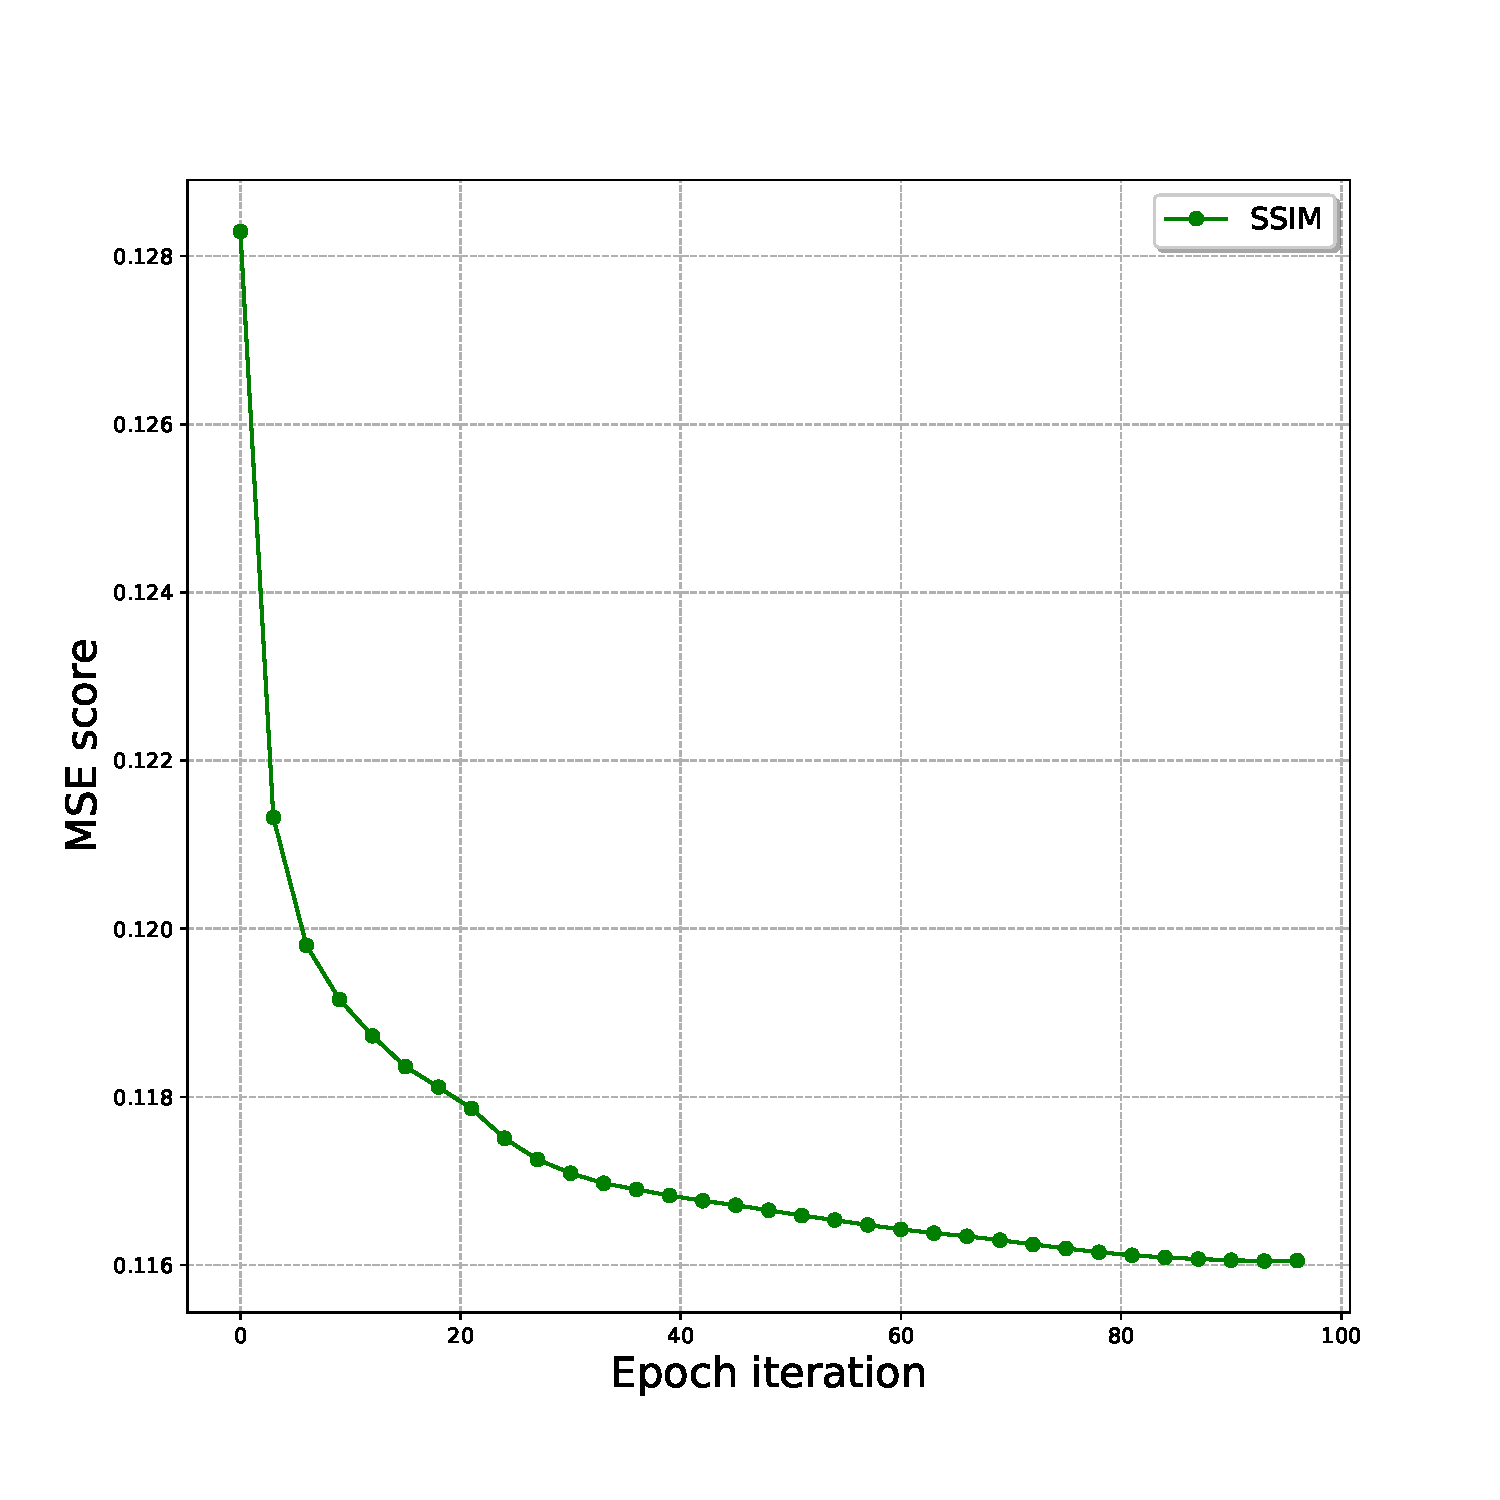
\includegraphics[width=1\textwidth]{resources/training-mse.pdf}
		\caption{Графік залежності штрафної функції MSE на тестовому датасеті від кількості епох. тренування.}
		\label{fig:attacks_bench}
		\endminipage\hfill
		\minipage[t]{0.49\textwidth}
		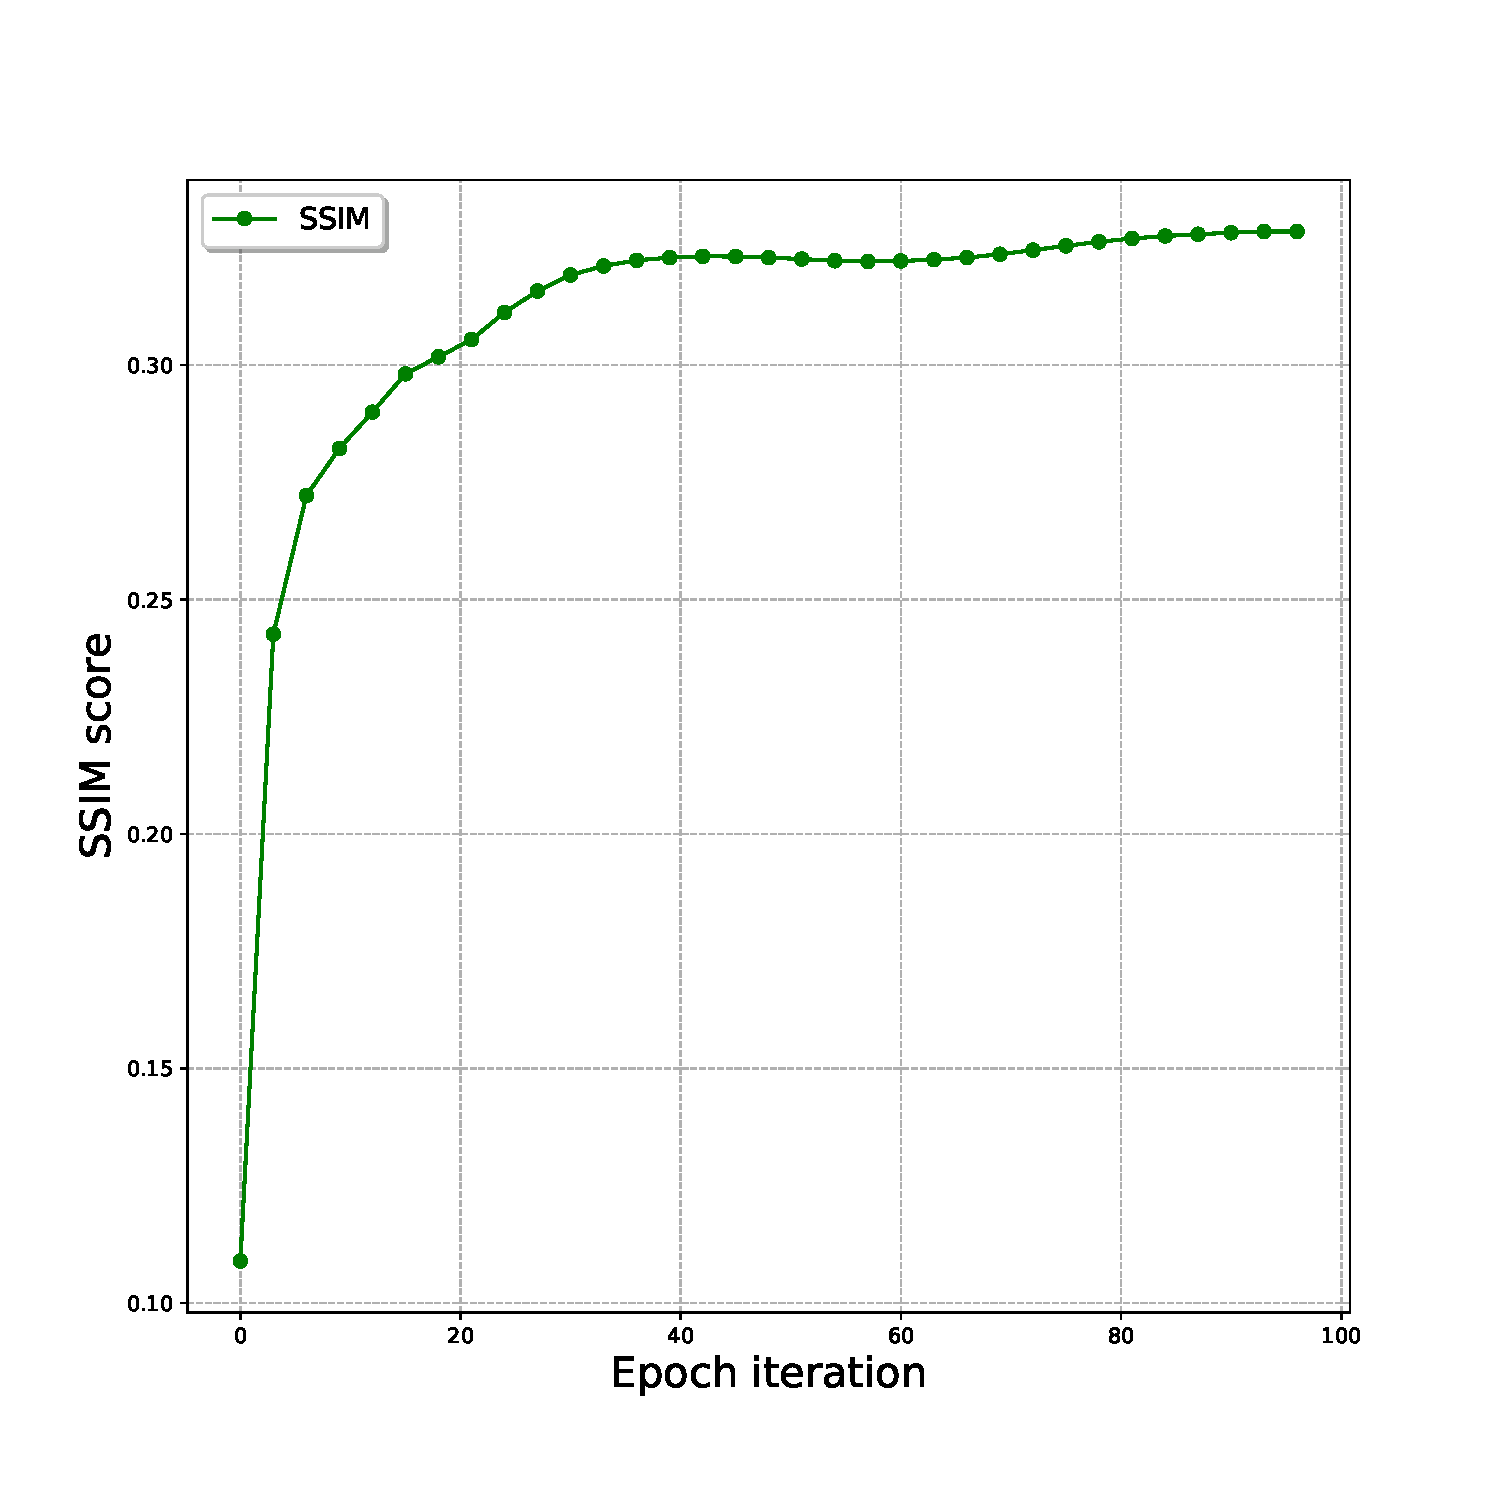
\includegraphics[width=1\textwidth]{resources/training-ssim.pdf}
		\caption{Графік залежності оцінки SSIM на тестовому датасеті від кількості епох тренування.}
		\label{fig:defenses_bench}
		\endminipage
	\end{figure}
	
	\begin{comment}
		\begin{tabular}{cccc}
			\hline & BN $\left(\beta+\gamma+\mu+\sigma^{2}\right)$ & Conv.filters & Total \\
			\hline conv1 & $64+64+64+64$ & $3 \times 3 \times 2 \times 64$ & 1408 \\
			conv2 & $64+64+64+64$ & $3 \times 3 \times 64 \times 64$ & 37120 \\
			$\lambda$ & & & 1 \\
			\hline
		\end{tabular}
	\end{comment}

	\subsection{Аналіз результатів}	
	TODO
	\begin{figure}[H]
		\centering
		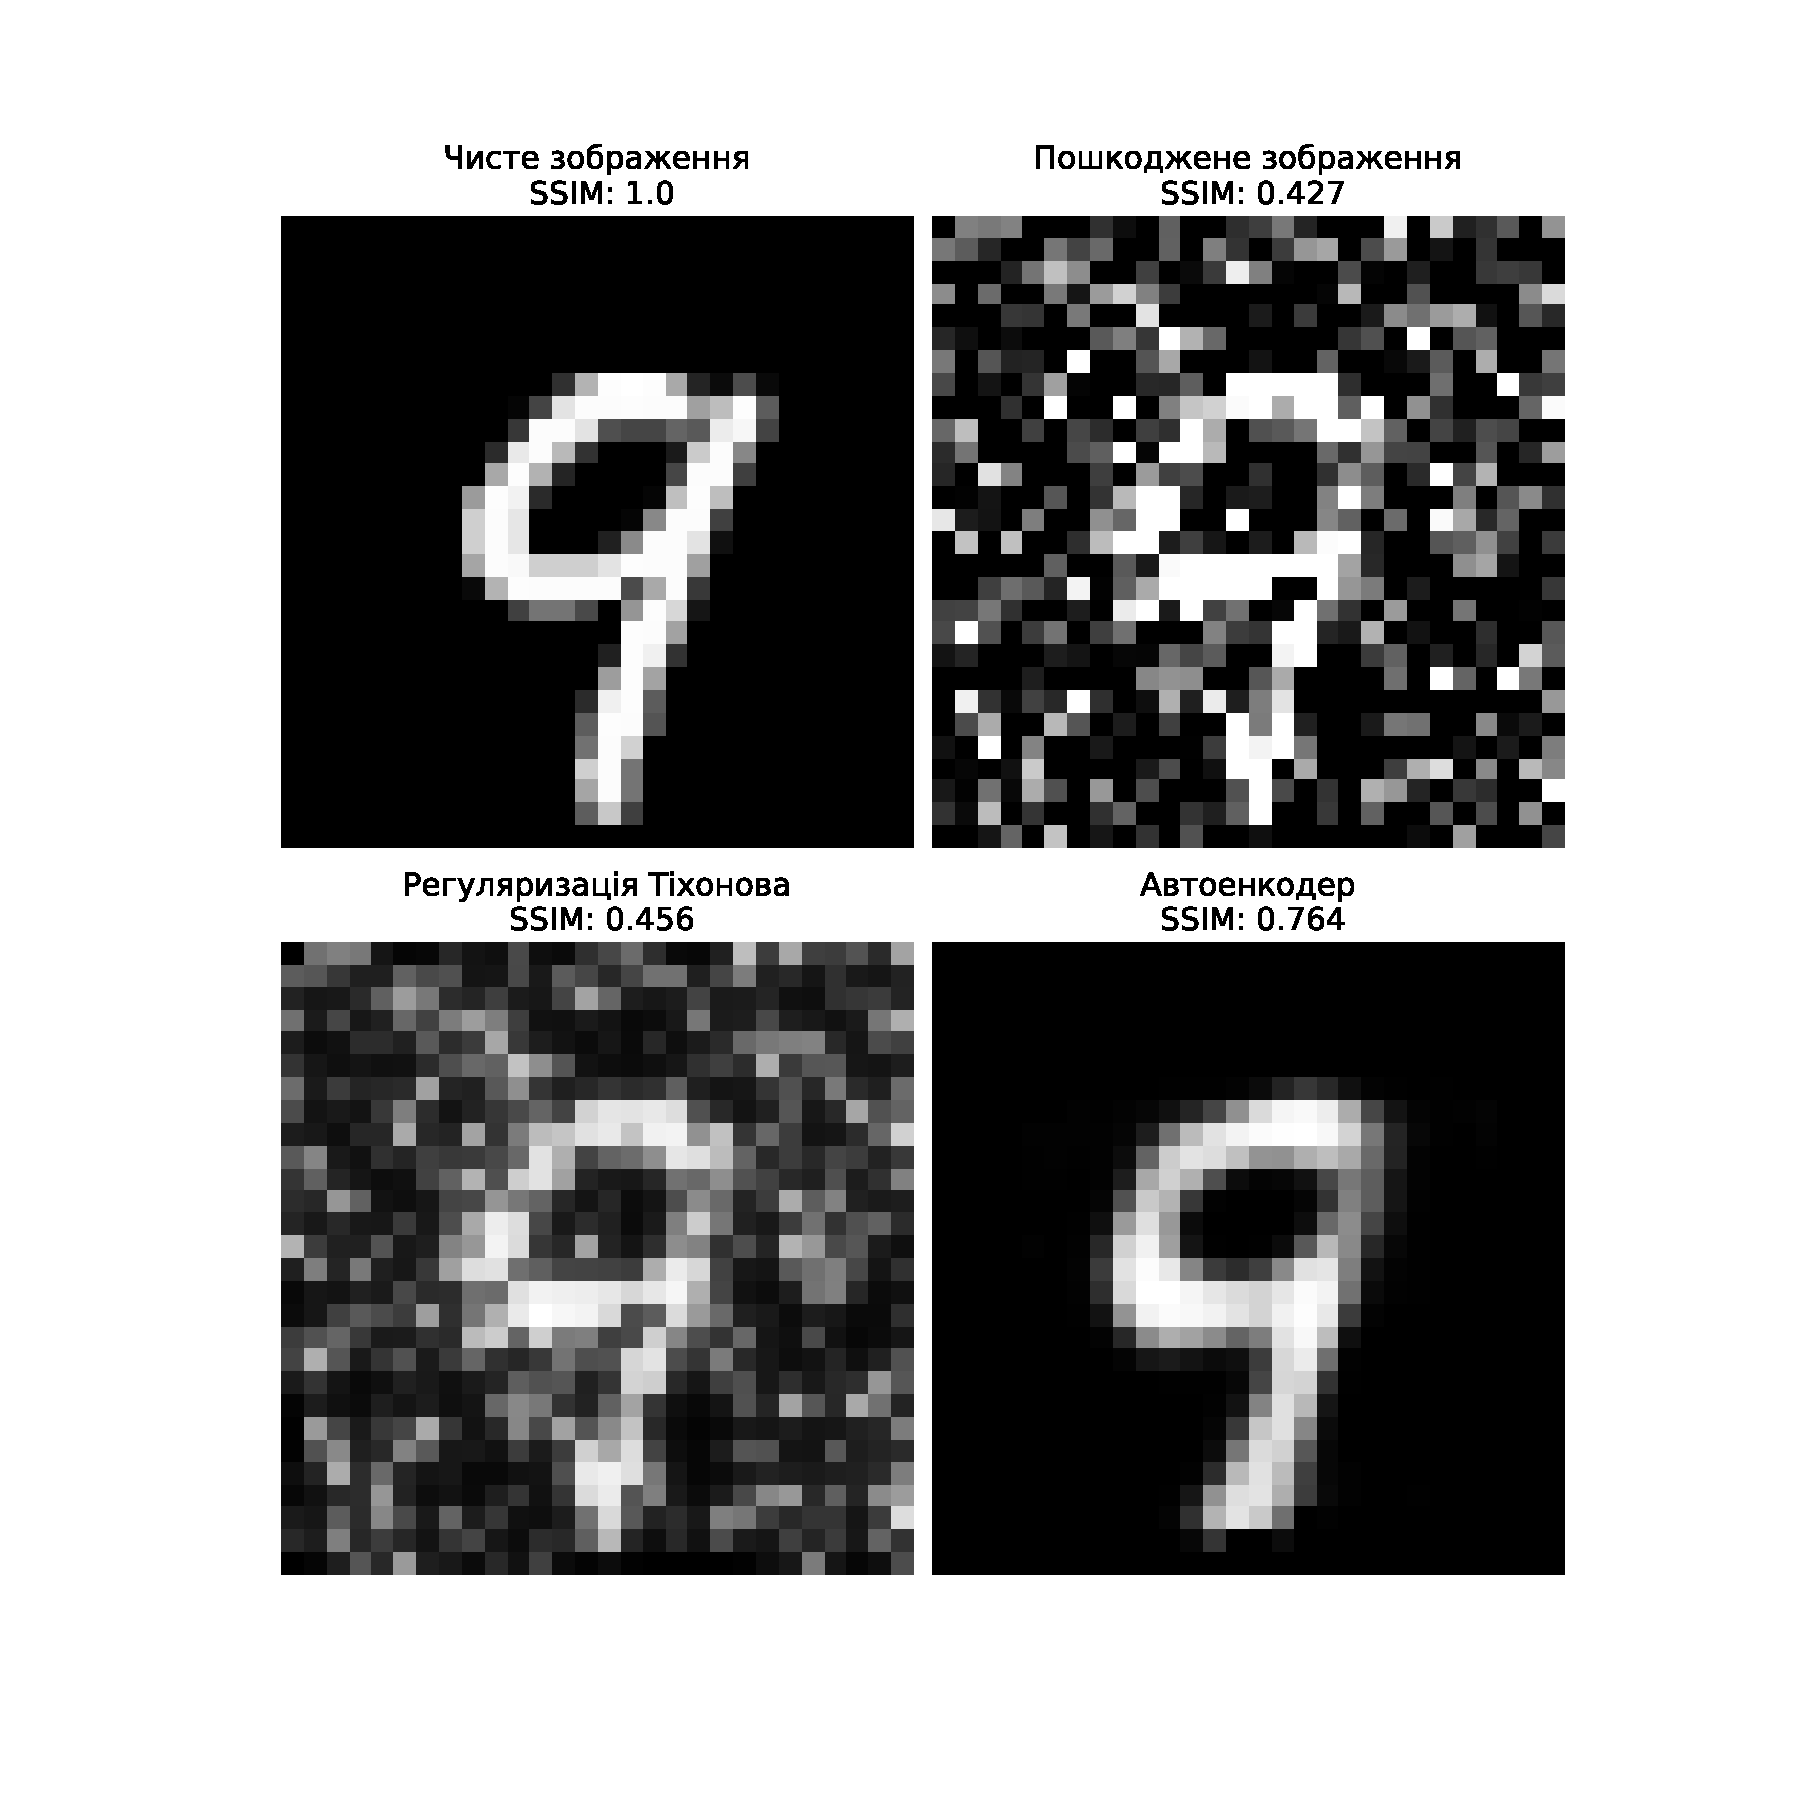
\includegraphics[width=1\textwidth]{resources/denoising_methods_comparation.pdf}
		\caption{}
		\label{fig:denoising-methods-comparation}
	\end{figure}
		
	% ============================================ %	
		
	% ============================================ %
	% Вступ
	
	%\newpage
	%\thispagestyle{empty}
	%\addcontentsline{toc}{section}{Вступ}
		
	%\newpage
	%\thispagestyle{empty}
	%\addtocontents{toc}{\protect\thispagestyle{empty}}
	\newpage
	\thispagestyle{empty}
	\addcontentsline{toc}{section}{Висновок}
	\section*{Висновок}
	TODO
	
	\newpage
	\thispagestyle{empty}
	\addcontentsline{toc}{section}{Додатки}
	\section*{Додатки}
	TODO
	
	%============================================ %
	
	\newpage
	\thispagestyle{empty}
	\addcontentsline{toc}{section}{Література}
	
	% Deep Learning Techniques for Inverse Problems in Imaging
	\nocite{ongie2020deep}
	\nocite{Goodfellow-et-al-2016}
	\nocite{Adler_2017}
	\nocite{NIPS2012_6cdd60ea}
	\nocite{raj2019ganbased}
	\nocite{Aggarwal_2019}
	\printbibliography[title={Література}]
	% ============================================ %
\end{document}